\documentclass[letterpaper, 11pt]{article}

% package to adjust page margins
\usepackage[
	inner = 0.75in,
	outer = 0.75in, 
	top = 1in,
	bottom = 1in,
	bindingoffset = 0.0 cm
	]{geometry}

\usepackage[backend=biber]{biblatex}	% bibliography package using biber instead of bibtex
\usepackage{amsmath}	% provides enhancement of math printout structure 
\usepackage{amssymb}	% provides an extended symbol collection
\usepackage{comment}	% package to use comment block
\usepackage{sectsty}	% to change the style of section headers
\usepackage{fancyhdr}	% to have fancy headers for each page
\usepackage{graphicx}	% allows you to import images
\usepackage{float}	% allows the control of float positions
\usepackage{imakeidx} 	% to create index pages
\makeindex[intoc] % creates index and toc

% allows for clickable references, also creates bookmarks that link to respective pages correctly
\usepackage[
	hidelinks, 
	bookmarksopen=true, 
	bookmarksnumbered=false, 
	bookmarksopenlevel=4,
	pdfview=Fit
	]{hyperref}

% List of macros
\newcommand{\fint}{\int_{-\infty}^{\infty}} % integral with infinite limits
\newcommand{\sed}[2]{#2_{0}e^{2\pi if_{0}#1}e^{-#1/T} \theta (#1)} % SED function
\newcommand{\fsum}[1]{\sum_{#1 = -\infty}^{\infty}} % infinite sum
\newcommand{\spf}[2]{\Delta #1 \fsum{#2} \delta (#1 - #2 \Delta #1)} % sampling function
\newcommand{\fourier}[2]{\mathcal{F}_{#1}[#2]} % Fourier transform notation
\newcommand{\ifourier}[2]{\mathcal{F}_{#1}^{-1}[#2]} % inverse FT notation
\newcommand{\ft}[3]{\fint #2 e^{-2\pi i#3#1} d#1} % Fourier transform 
\newcommand{\ift}[3]{\fint #2 e^{2\pi i#1#3} d#1} % Inverse Fourier transform 
\newcommand{\conv}[4]{\fint #3(#2)#4(#1 - #2) d#2} % Convolution
\newcommand{\ssum}[1]{\sum_{#1 = 0}^{N - 1}} % sum from 0 to N-1
\newcommand{\dft}[3]{\ssum{#1} #2 e^{-2\pi i#3#1/N}} % DFT 
\newcommand{\idft}[3]{\frac{1}{N}\ssum{#1} #2 e^{2\pi i#3#1/N}} % Inverse DFT 
\newcommand{\dtft}[3]{\fsum{#1} #2 e^{-2\pi i#3#1}}

% Numbering equation and figure with section number
\numberwithin{equation}{section}
\numberwithin{figure}{section}
\numberwithin{table}{section}

% Centering section titles
\sectionfont{\centering}

% Adding bib file
\addbibresource{ft.bib}

\begin{document}
% Front cover page with title and name
\pdfbookmark[0]{Cover}{cover}
\begin{titlepage}
	\begin{center}
		% \vfill must have preceding text line
		\Huge{\bfseries Fourier Transform}\vfill 
	\end{center}

	\begin{flushright}
		Sejin Nam\\
		University of Hawaii at Manoa
	\end{flushright}
\end{titlepage}

\begin{comment} % commenting out standard title page
\title{Fourier Transform}
\author{Sejin Nam}
\date{May 20}
\maketitle
\thispagestyle{empty}
\clearpage
\end{comment}

% page numbering in roman numerals
\pagenumbering{roman}

% Preface
\pdfbookmark[1]{Preface}{preface}
\section*{\centering Preface}
Fourier transform is a mathematical transformation, in the context of my exposition, that maps one function in time domain into another function in frequency domain. In order for a function to have its Fourier transform, the function needs to be Schwartz. However, in Physics, we extend the notion of function to a more generalized case, called a generalized function. In a generalized function space, we allow more flexibility so that functions like Dirac delta function can have the Fourier transform even though such function is not Riemann integrable. In this article I will assume that every function that is discussed has its Fourier transform. I will call Fourier transform FT in short, and there are two types of FT: continuous and discrete. Discrete FT is of great importance in many modern data processing application as data can only be recorded in discrete and finite amount. Also, modern computers are digital, meaning they perform computation in discrete manner. In this article, I'll discuss a continous case first before moving onto the discrete case.
\cleardoublepage

% Table of Contents
\pdfbookmark[1]{Table of Contents}{toc}
\tableofcontents
\clearpage

% use fancyhdr
\pagestyle{fancy}

% First Section: prerequisite mathematics
\pagenumbering{arabic}
\section{Prerequisite Mathematics}
A few prerequisite mathematics will be discussed here first in anticipation of their requirements in the discussion of subsequent sections of Fourier transform. In this article, it is implied that all the functions discussed are generalized functions, \(\mathbb{R} \mapsto \mathbb{C} \) (the domain is either \(t\) or \(f\)), and infinitely differentiable unless stated otherwise. Also, all the definite integrals and infinite sums are assumed to be convergent.  

% 1.1 Dirac Delta Functio
\subsection{Dirac Delta Function}\index{Dirac Delta function}
The Dirac Delta function, \(\delta (t)\), has the following properties:
\begin{align}
	\delta (t)	&=\begin{cases}
			\infty, & \text{if } t = 0 \\
			0,	& \text{otherwise}
	\end{cases}\\
		1	&= \fint \delta (t) dt
\end{align}
(In my discussion of function, \(t\) variable represents time physically). It is easy to check that:
\begin{align}
	f(a)		&= \fint f(t) \delta (t) dt\\
	\delta (t)	&= \delta (-t)\\
	\delta (at)	&= \frac{\delta (t)}{|a|}
\end{align}
Also, the following integral is the Dirac Delta function as well:
\begin{align}
	\delta (t)	&= \ift{f}{}{t}
	\label{eq:dirac}
\end{align}
with the understanding that the Dirac Delta function has meaning only when under an integral sign \cite{arfken}. The above relations will be used throughout the discussion of this article.


% 1.2 Sampling function  
\subsection{Sampling function}\index{Sampling function}
The sampling function, denoted as \(u(t)\), with the \emph{sampling interval} \(\Delta t\) \index{Sampling interval} is as follows:
\begin{equation}
	\begin{aligned}[b]
		u(t) = \spf{t}{n}
	\end{aligned}
\end{equation}
The function is periodic with the period being the sampling interval. 

% 1.3 Convolution
\subsection{Convolution}\index{Convolution}
Convolution is a mathematical operation on two functions (say \(x(t)\) and \(y(t)\)) that outputs another function. The symbol for the operator is \(*\). The definition is as follows:
\begin{equation}
	\begin{aligned}[b]
		x(t)*y(t)
			&= \conv{t}{\tau}{x}{y}
			\label{eq:convolution}
	\end{aligned}
\end{equation}
\((x*y)(t)\) notation is also used. The term \emph{convolution} refers to both the result function and to the process of computing it. The table \ref{tab:convolution} lists a few properties of Convolution \cite{arfken}.
\begin{table}
	\centering
	\caption[optional argument]{Properties of Convolution}
	\begin{tabular}{|l|l|}
		\hline
		Property	& Mathematical Expression\\
		\hline
		Commutativity	& \(x*y = y*x\) \\
		\hline
		Associativity	& \(x*(y*z) = (x*y)*z \) \\
		\hline
		Distributivity	& \(x*(y + z) = x*y + x*z \) \\
		\hline
		Multiplicative identity	& \(x*\delta = x \)\\
		\hline
		Complex Conjugation	& \(\overline{x*y} = \overline{x}*\overline{y}\) \\
		\hline
		Differentiation	& \((x*y)' = x'*y = x*y' \) \\
		\hline
		Integration	& \(\int_{\mathbb{R}}(x*t)(t) dt
					= \int_{\mathbb{R}} x(t) dt
					  \int_{\mathbb{R}} y(t) dt\) \\
		\hline
	\end{tabular}
	\label{tab:convolution}
\end{table}

% 1.4 Kronecker delta
\subsection{Kronecker delta}\index{Kronecker delta}
Suppose \(i\) and \(j\) are integers. Then a Kronecker delta is defined as:
\begin{equation}
	\begin{aligned}[b]
		\delta_{ij}	&=\begin{cases}
				1, 	&\text{if } i=j\\
				0,	&\text{otherwise}
		\end{cases}
	\end{aligned}
\end{equation}
Now consider two integers \(n\) and \(p\) where \(0 \leq n,p \leq N-1\). Also consider the following sum:
\begin{equation}
	\begin{aligned}[b]
		\frac{1}{N}\ssum{k} e^{2\pi ik(n - p)/N} 
	\end{aligned}
\end{equation}
If \(n = p\), \(e^{-2\pi ik(n - p)/N} = 1\), which means
\begin{equation}
	\begin{aligned}[b]
		\frac{1}{N}\ssum{k} e^{2\pi ik(n - p)/N}
			&= \frac{1}{N}\ssum{k} 1\\
			&= 1
	\end{aligned}
\end{equation}
If \(n \neq p\), then \(2\pi i(n - p)/N \neq 0\). Thus, it follows that
\begin{equation}
	\begin{aligned}[b]
		\frac{1}{N}\ssum{k} e^{2\pi ik(n - p)/N}
			&= \frac{1}{N}\ssum{k} (e^{2\pi i(n - p)/N})^{k}\\
			&= \frac{1}{N}\frac{1 - e^{2\pi i(n - p)}}{1 - e^{2\pi i(n - p)/N}}
	\end{aligned}
\end{equation}
Where I used the geometric series formula:
\begin{equation}
	\begin{aligned}[b]
		\ssum{k} a^{k} = \frac{1 - x^{N}}{1 - x}
	\end{aligned}
\end{equation}
with \(a \neq 1\). Also, we know that \(e^{2\pi i(n - p)} = 1\) because \(n - p\) is an integer and \(e^{2\pi im} = 1\) for any integer \(m\). Therefore, it follows that if \(n \neq p\),
\begin{equation}
	\begin{aligned}[b]
		\frac{1}{N}\ssum{k} e^{2\pi ik(n - p)/N}
			&= \frac{1}{N}\frac{1 - e^{2\pi i(n - p)}}{1 - e^{2\pi i(n - p)/N}}\\
			&= 0
	\end{aligned}
\end{equation}
Thus, the above sum satisfies the Kronecker delta condition. In other words,
\begin{equation}
	\begin{aligned}[b]
		\delta_{np}	&= \frac{1}{N}\ssum{k} e^{2\pi ik(n - p)/N}
				\label{eq:kronecker}
	\end{aligned}
\end{equation}

% 1.5 Sinusoidal expoential decay function
\subsection{Sinusoidal exponential decay function}\index{SED}
Sinusoidal exponential decay function (I call it SED) is as follows:
\begin{equation}
	\begin{aligned}[b]
		x &= x_{0}\cos{(2\pi f_{0}t)}e^{-t/T} \theta(t)
		\label{eq:rsed}
	\end{aligned}
\end{equation}
where \(\theta (t)\) is a heaviside step function and \(T > 0\) (SED function plot is given in figure \ref{fig1}). you can have sine instead of cosine in the above expression. for our discussion, sed of choice is combination of sine and cosine exponential decays in complex form:
\begin{equation}
	\begin{aligned}[b]
		x	&= x_{0}\cos{(2\pi f_{0}t)}e^{-t/T} \theta(t)+ i x_{0}\sin{(2\pi f_{0}t)}e^{-t/T} \theta(t)\\
			&= (\cos{(2\pi f_{0}t)} +i \sin{(2\pi f_{0}t)})x_{0}e^{-t/T} \theta(t) \\
			&= \sed{t}{x}
			\label{eq:sed}
	\end{aligned}
\end{equation}
The real part of \eqref{eq:sed} is simply \eqref{eq:rsed}.

% 1.6 End of the section

% figure for sed function
\begin{figure}[H]
	\centering
	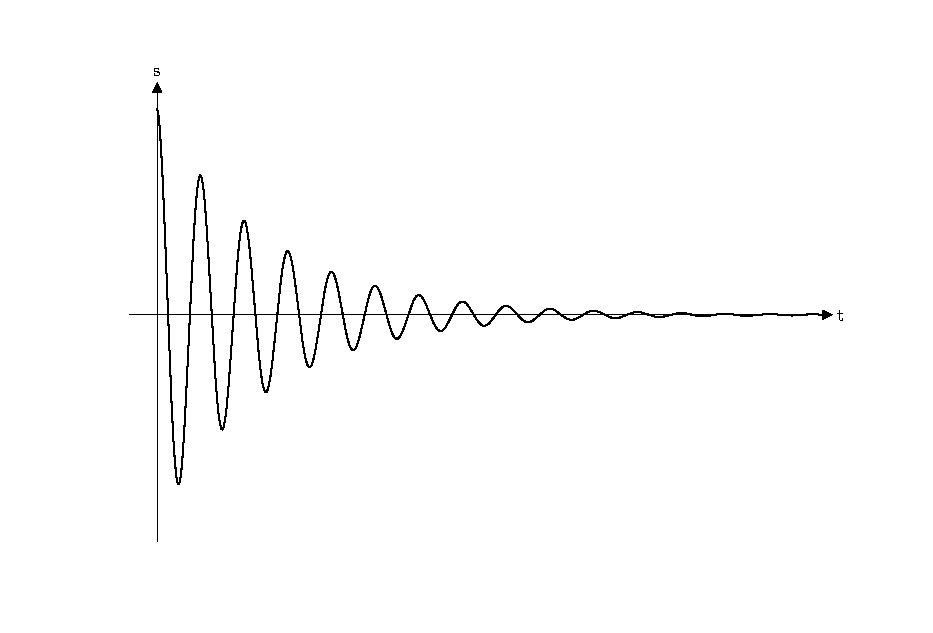
\includegraphics[height=5in]{sed.eps}
	\caption{sed function plot, s vs. t}
	\label{fig1}
\end{figure}

% Second Section: Continuou Fourier transform
\clearpage
\section{Continuous Fourier Transform}\index{Fourier transform}
Continuous FT transforms a complex-valued function in \(t\) to another complex-valued function in \(f\). Also, as we will see, the inverse FT of the function in \(f\) will recover the original function in \(t\). 

% 2.1 Definition of Fourier transform
\subsection{Definition of Fourier transform}
Consider a function of \(t\), \(x(t)\). The continuous FT of \(x\), \(X(f)\), is as follows:
\begin{equation}
	\begin{aligned}[b]
		X(f)	&=\fourier{t}{x} \\
			&=\ft{t}{x(t)}{f}
	\end{aligned}
\end{equation}
It is sometimes called continuous-time Fourier transform (CTFT) to emphasize that \(t\) variable represents physical continuous time in an application. The domain of \(X(f)\), \(f\), is also in \(\mathbb{R}\). (in my discussion \(t\) and \(f\) represent time and frequency respectively). \(\fourier{t}{x}(f)\) notation can be used to explicitly indicate that \(x\) is transformed into \(f\) domain. It is easy to see that if \(a\) is a constant, then \(\fourier{t}{ax} = a \fourier{t}{x}\). You can also perform inverse FT on \(X\), which is:
\begin{equation}
	\begin{aligned}[b]
		\ifourier{f}{X}	&= \ift{f}{X(f)}{t} \\
				&= \ift{f}{\left ( \ft{\tau}{x(\tau)}{f}\right )}{t} \\
				&= \fint x(\tau) \fint e^{2\pi if(t - \tau)} df d\tau \\
				&= \fint x(\tau) \delta (t - \tau) d\tau \\
				&= x(t)
	\end{aligned}
\end{equation}
where I used \eqref{eq:dirac} orthogonality relation .We will continue to use the notation \(x(t)\) and \(X(f)\) as an example of FT pair throughout the discussion (they are called 'Fourier pair'). It is also easy to see that the inverse FT of one is the Dirac Delta function \cite{james}.

% 2.2 FT with the extra phase factor
\subsection{FT with the extra phase factor}
Consider another function, \(e^{2\pi i f_{0} t}x(t)\). The FT of it is:
\begin{equation}
	\begin{aligned}[b]
		\fourier{t}{e^{2\pi i f_{0} t}x(t)}
			&= \ft{t}{e^{2\pi i f_{0} t}x(t)}{f}\\
			&= \ft{t}{x(t)}{(f - f_{0})}\\
			&= \fourier{t}{x}(f - f_{0})\\
			&= X(f - f_{0})
	\end{aligned}
\end{equation}
It is simply the FT of \(x\) in \(f - f_{0}\) in domain. By the same token, it is easy to see that \(\fourier{t}{x(t - \tau)} = e^{-2\pi i f\tau}X(f)\). A list of FT properties is in the table \ref{tab:ft} \cite{arfken}:
\begin{table}
	\centering
	\caption[optional argument]{Properties of Fourier transform}
	\begin{tabular}{|l|l|}
		\hline
		Property		& Mathematical Expression\\
		\hline
		Linearity		& \(\fourier{t}{ax + by} = aX + bY\) \\
		\hline
		Shift in time		& \(\fourier{t}{x(t -\tau)} = e^{-2\pi if\tau}X(f)\)\\
		\hline
		Phase factor		& \(\fourier{t}{e^{2\pi i f_{0} t}x(t)} = X(f - f_{0})\)\\
		\hline
		Scaling in time domain	& \(\fourier{t}{x(at)} = \frac{1}{a}X(f/a)\)\\
		\hline
		Complex conjugation	& \(\overline{\fourier{t}{x}} = \overline{X(-f)}\) \\
		\hline
		FT of Convolution	& \(\fourier{t}{x*y} = X(f)Y(f) \)\\
		\hline
		FT of product		& \(\fourier{t}{xy} = X(f)*Y(f) \)\\
		\hline
	\end{tabular}
	\label{tab:ft}
\end{table}

% 2.3 Poisson Summation Formula
\subsection{Poisson Summation Formula}\index{Poisson Summation Formula}
Consider a Fourier pair \(x(t)\) and \(X(f)\). Then the Poisson Summation formula states that \cite{stein}:
\begin{equation}
	\begin{aligned}[b]
		\fsum{n} x(n)	&= \fsum{k} X(k)
	\end{aligned}
\end{equation}
For example, if \(x(n) = e^{2 \pi ian}\), then we know that the FT of \(x(n)\) is:
\begin{equation}
	\begin{aligned}[b]
		X(k)	&= \fourier{n}{x}(k) \\
			&= \fourier{n}{e^{2 \pi ian} \times 1}(k) \\
			&= \fourier{n}{1}(k - a) \\
			&= \delta (k - a)
	\end{aligned}
\end{equation}
Thus, according to the Poisson Summation formula, it follows that:
\begin{equation}
	\begin{aligned}[b]
		\fsum{n} e^{2 \pi ian}
			&= \fsum{k} \delta (k - a)
			\label{eq:poisson}
	\end{aligned}
\end{equation}

% 2.4 FT of the sampling function
\subsection{FT of the sampling function}
Suppose \(u(t)\) is the sampling function with the sampling interval \(\Delta t\). Then the FT of \(u\) is:
\begin{equation}
	\begin{aligned}[b]
		\fourier{t}{u}
			&= \ft{t}{u(t)}{f} \\
			&= \ft{t}{\spf{t}{n}}{f} \\
			&= \Delta t \fsum{n} e^{-2\pi ifn\Delta t} \fint \delta (t - n \Delta t) dt \\
			&= \Delta t \fsum{n} e^{-2\pi ifn\Delta t}
	\end{aligned}
\end{equation}
By applying \eqref{eq:poisson}, we can deduce that:
\begin{equation}
	\begin{aligned}[b]
		\fourier{t}{u}
			&= \Delta t \fsum{n} e^{-2\pi ifn\Delta t} \\
			&= \Delta t \fsum{k} \delta (k + f \Delta t)\\
			&= \fsum{k} \delta (f + kf_{s})
	\end{aligned}
\end{equation}
Where \(f_{s} = 1/\Delta t\) is called a \emph{sampling rate}\index{Sampling rate}.

% 2.5 FT of s multiplied by u
\subsection{FT of product of \(u(t)\) and \(s(t)\)}\label{sec:su}
Consider an arbitrary function \(s(t)\). Let \(x(t) = s(t)u(t)\). The FT of \(x(t)\) is then:
\begin{equation}
	\begin{aligned}[b]
		\fourier{t}{x}
			&= \ft{t}{s(t)u(t)}{f}\\
			&= \ft{t}{s(t) \spf{t}{n}}{f}\\
			&= \fsum{n} s(n \Delta t) e^{-2\pi ifn\Delta t} \Delta t 
			   \fint \delta (t - n\Delta t) dt\\
			&= \fsum{n} s(n \Delta t) e^{-2\pi ifn\Delta t} \Delta t 
			\label{eq:ftsu}
	\end{aligned}
\end{equation}
If \(\Delta t \to 0\), the above infinite sum becomes FT of \(s(t)\). 

% 2.6 FT of Convolution
\subsection{FT of Convolution}
Consider the convolution of two functions \(x(t)*y(t)\). The FT of it is:
\begin{equation}
	\begin{aligned}[b]
		\fourier{t}{(x*y)(t)}
			&= \ft{t}{(x*y)(t)}{f}\\
			&= \ft{t}{\left (\conv{t}{\tau}{x}{y} \right )}{f}\\ 
			&= \fint x(\tau) \left (\fint y(t - \tau) e^{-2\pi ift} dt \right ) d\tau\\
			&= \fint x(\tau) \left ( e^{-2\pi if\tau}\fourier{f}{Y} \right )d\tau\\ 
			&= \fourier{f}{Y} \ft{\tau}{x(\tau)}{f}\\
			&= \fourier{f}{X} \fourier{f}{Y}\\
			&= X(f)Y(f)
	\end{aligned}
\end{equation}
by the same token,
\begin{equation}
	\begin{aligned}[b]
		\fourier{t}{x(t)y(t)}
			&= X(f)*Y(f)
			\label{eq:ftconv}
	\end{aligned}
\end{equation}
Here you can see convolutions can be used to make FT easier \cite{james}.

% 2.7 FT of s and u again
\subsection{FT of \(s(t)u(t)\) again}
Consider \(x(t) = s(t)u(t)\) discussed in section \ref{sec:su} again. We already showed that \(X(f)\) is \eqref{eq:ftsu}. We can also see that, by applying \eqref{eq:ftconv}, 
\begin{equation}
	\begin{aligned}[b]
		\fourier{t}{su}
		&= S(f)*U(f)\\
		&= \conv{f}{\xi}{S}{U}\\
		&= \fint S(\xi) 
		   \left (\fsum{k} \delta (f + kf_{s}- \xi) \right ) d\xi\\
		&= \fsum{k} S(f + kf_{s}) \fint \delta (f + kf_{s} - \xi) d\xi\\
		&= \fsum{k} S(f + kf_{s}) 
	\end{aligned}
\end{equation}
In other words, 
\begin{equation}
	\begin{aligned}[b]
		\fsum{n} s(n \Delta t) e^{-2\pi ifn\Delta t} \Delta t 
			&= \fsum{k} S(f + kf_{s}) 
			\label{eq:ftsu1}
	\end{aligned}
\end{equation}

% 2.8 FT of SED function 
\subsection{FT of SED}
We will now consider a specific function, in this case, SED function discussed in section 1, \(x = \sed{t}{x}\). The FT of \(x\) is (with \(1/T = r\)) as follows:
\begin{equation}
	\begin{aligned}[b]
		X(f)	&= \fourier{t}{x}\\
			&= \fourier{t}{\sed{t}{x}}\\
			&= x_{0}\fourier{t}{e^{-rt} \theta (t)}(f - f_{0})\\
			&= \frac{x_{0}}{r + 2\pi i(f - f_{0})} \\
			\gdef\temp{r^2 + 4\pi^{2}(f - f_{0})^2} % temporary macro
			&= x_{0}\frac{r - 2\pi i(f - f_{0})}{\temp}\\
			&= x_{0}\left[\frac{r}{\temp} + i\frac{2\pi(f_{0} - f)}{\temp} \right]
	\end{aligned}
\end{equation}
The maximum of \(X(f)\), which is at \(f_{0}\), is \(x_{0}/r\).
% 2.9 End of the section 2
\clearpage

% Third section: Discrete Fourier transform
\section{Discrete Fourier transform}
Unlike continuous FT, discrete FT, or DFT in short, converts a finite sequence \(\{x_{n}\}_{n=0}^{N-1} \), instead of continuous function, into an element of another finite sequence \( \{X_{n}\}_{n=0}^{N-1} \). As you can see from the above sequences, there are \(N\) elements of both \(x\) and \(X\) respectively. From now on it is implied that all the sequences without explicit subscripts and superscripts run from \(n=0\) to \(n=N-1\).   

% 3.1 Definition of DFT
\subsection{Definition of DFT}\index{discrete Fourier transfomr}
Consider a sequence \(\{x_{n}\}\). Then DFT of \(x_{n}\) is:
\begin{equation}
	\begin{aligned}[b]
		X_{k}	&= \fourier{}{x_{n}}\\
			&= \dft{n}{x_{n}\,}{k}
	\end{aligned}
\end{equation}
The inverse DFT of \(X_{k}\) is:
\begin{equation}
	\begin{aligned}[b]
		\ifourier{}{X_{k}}
			&= \idft{k}{X_{k}}{n}\\
			&= \idft{k}{\dft{p}{x_{p}\,}{k}}{n}\\
			&= \ssum{p} x_{p} \frac{1}{N}\ssum{k} e^{2\pi ik(n-p)/N}\\
			&= \ssum{p} x_{p} \delta_{np}\\
			&= x_{n}
	\end{aligned}
\end{equation}
Where I used the orthogonal relation \eqref{eq:kronecker}\cite{james}. There is another version of DFT called discrete-time Fourier transform (DTFT in short)\index{discrete-time Fourier transform}. The only difference is that the sum runs from negative infinity to positive infinity with a continuous domain (the example is \eqref{eq:ftsu}, which is DTFT of \(\Delta t\cdot s(n\Delta t)\) whose element of the domain is \(f\Delta t\)). 

% 3.2 Approximation of DFT
\subsection{Approximation of DFT}
Consider a function \(x(t)\) and let \(x_{n} = x(n\Delta t)\). Then its DTFT is:
\begin{equation}
	\begin{aligned}[b]
		X(a) = \dtft{n}{x_{n}}{a} 
	\end{aligned}
\end{equation}
Now suppose that \(x(t) = 0\) for all \(t < 0\) and \(x(t) \approx 0\) after some time \(t = N\Delta T\) where \(N \in \mathbb{N}\) (in other words, \(x_{n} \approx 0\) for \(n \ge N\)). And we are only interested in \(a\) values such that \(a = k/N\) where \(k\) is an integer and \(0 \leq k \leq N - 1\). Then
\begin{equation}
	\begin{aligned}[b]
		X_{k} 	&= X(k/N)\\
			&= \dtft{n}{x_{n}}{(k/N)}\\
			&\approx \dft{n}{x_{n}}{k}
	\end{aligned}
\end{equation}
Which is just DFT of \(x_{n}\). We can take this analogy further with CTFT. Consider \(x(t)=f_{s} s(t)u(t)\) such that \(s(t)\) has the properties that \(x(t)\) has described above (for example, SED function) and \(u(t)\) is a sampling function with the sampling rate \(f_{s}\). Then we know from \eqref{eq:ftsu} that
\begin{equation}
	\begin{aligned}[b]
		\fourier{t}{x}
			&= \fsum{n} s_{n} e^{-2\pi ifn\Delta t} 
	\end{aligned}
\end{equation}
Where \(s_{n} = s(n\Delta t)\). If we are only interested in frequencies \(f = kf_{s}/N\) where \(k\) is an integer and \(0 \leq k \leq N - 1\), then with the properties of \(s\), we have
\begin{equation}
	\begin{aligned}[b]
		\fsum{n} s_{n} e^{-2\pi ifn\Delta t}
			&\approx \dft{n}{s_{n}}{k}
	\end{aligned}
\end{equation}
In other words, by applying \eqref{eq:ftsu1}, we have
\begin{equation}
	\begin{aligned}[b]
		S_{k}	&= \dft{n}{s_{n}}{k}\\
			&\approx f_{s}\fsum{p} S(f_{k} + pf_{s}) 
	\end{aligned}
\end{equation}
Where \(f_{k} = kf_{s}/N\). Here, \(S_{k}\) is DFT of \(s_{n}\) and \(S(f)\) is CTFT of \(s(t)\).
% Bibliography and index
\clearpage
\pagestyle{plain}
\printbibliography
\addcontentsline{toc}{section}{References}
\printindex
\end{document}
